%%=============================================================================
%% Methodologie
%%=============================================================================

\chapter{\IfLanguageName{dutch}{Methodologie}{Methodology}}%
\label{ch:methodologie}



%% TODO: In dit hoofstuk geef je een korte toelichting over hoe je te werk bent
%% gegaan. Verdeel je onderzoek in grote fasen, en licht in elke fase toe wat
%% de doelstelling was, welke deliverables daar uit gekomen zijn, en welke
%% onderzoeksmethoden je daarbij toegepast hebt. Verantwoord waarom je
%% op deze manier te werk gegaan bent.
%% 
%% Voorbeelden van zulke fasen zijn: literatuurstudie, opstellen van een
%% requirements-analyse, opstellen long-list (bij vergelijkende studie),
%% selectie van geschikte tools (bij vergelijkende studie, "short-list"),
%% opzetten testopstelling/PoC, uitvoeren testen en verzamelen
%% van resultaten, analyse van resultaten, ...
%%
%% !!!!! LET OP !!!!!
%%
%% Het is uitdrukkelijk NIET de bedoeling dat je het grootste deel van de corpus
%% van je bachelorproef in dit hoofstuk verwerkt! Dit hoofdstuk is eerder een
%% kort overzicht van je plan van aanpak.
%%
%% Maak voor elke fase (behalve het literatuuronderzoek) een NIEUW HOOFDSTUK aan
%% en geef het een gepaste titel.





\section{Renaissance benchmark suite}
Voor de Java programma's maken we gebruik van de \textit{Renaissance benchmark suite}.
Dit is een collectie van enkele \textit{real-world} Java programma's, hiermee wordt bedoeld dat dit programma's zijn die een degelijke hoeveelheid instructies uitvoeren, en in een werkelijke business context zouden gebruikt kunnen worden. 
Verder maken sommige programma's gebruik van bepaalde populaire Java frameworks.



Het gebruiken van deze benchmark suite maakt het mogelijk om Garbage Collection data te verzamelen met een grote waaier aan diverse programma's, zodanig dat we een goed beeld krijgen van de invloed van Garbage Collection in verschillende reële situaties.
Aangezien de te draaien benchmark programma's op zowel de mainframe als niet-mainframe systeem dezelfde bewerkingen uitvoeren betekent dit dat er geen invloed op de Garbage Collection zal zijn vanwege een verschil in het programma zelf.


De benchmark suite is ook garbage collector agnostisch, de benchmark suite kan met om het even welke garbage collector policy uitgevoerd worden.


Eens we de data verkregen hebben zullen we vergelijkingstabellen en grafieken opstellen om een analyse uit te kunnen voeren.

\newpage
\begin{table}[]
\section{Systeem informatie}

De volgende tabel geeft een overzicht van de specificaties van beide systemen;


    \caption{systeem informatie}
    \label{tab:Systeeminformatie}
    \begin{tabular}{@{}lll@{}}
        \toprule
        & Mainframe   & Niet-mainframe \\
        architectuur                                                       & s390x       & amd64          \\
        CPU's                                                              & 5           & 8              \\
        \begin{tabular}[c]{@{}l@{}}Operating\\ System\end{tabular}         & z/OS        & Windows 10     \\
        OS Versie                                                          & 02.04.00    & 10.0           \\
        \begin{tabular}[c]{@{}l@{}}Fysieke geheugen\\ (Gigabytes)\end{tabular} & 48,42 & 25,72    \\ \midrule
        &             &               
    \end{tabular}
\end{table}







\chapter{Uitvoering}
\label{ch:uitvoering}

Om deze Java applicaties uit te voeren maken we gebruik van de IBM Semeru Runtimes, dit is een open source Java SDK ontwikkeld door IBM.
Een Java SDK is een collectie van middelen om software voor Java te ontwikkelen.
De Openj9 JVM wordt meegeleverd met de Semeru SDK, deze zal zorgen voor de effectieve uitvoering van de programma's.
We zullen de IBM Semeru Runtimes SDK op zowel mainframe als niet-mainframe gebruiken.



Voor de uitvoering zullen we 4 benchmark programma's gebruiken, namelijk;


\begin{enumerate}
    \item \textit{akka-uct}
    
    Gebruikt de Akka library om de \textit{Unbalanced Cobwebbed Tree actor } workload uit te voeren.
    
    
    \item \textit{future-genetic}
    
    Voert een genetische algoritme uit met behulp van de \textit{Jenetics library}.
    
    \item \textit{dotty}
    
    Draait de dotty compiler op een aantal \textit{source code} bestanden.
    
    \item \textit{finagle-chirper}
    
    Maakt gebruik van Twitter Finagle om een webservice te simuleren.
    
    
\end{enumerate}


\section{Parameters}
Voor het uitvoeren van de benchmarks zullen we enkele Java parameters instellen.
De parameters zullen nu opgesomd worden.

\begin{enumerate}
    
    \item \textit{-Xms4096m}
    
    Deze parameter bepaalt de initiële grootte van de heap, ingezet op 4096 megabyte.
    
    
    \item \textit{-Xmx4096m}
    
    De maximale grootte van de heap, gezet op 4096 megabyte.
    Door de maximale en minimale \textit{heapsize} op dezelfde waarde in te stellen garanderen we dat de heap grootte gelijk blijft, en zo de voorspelbaarheid dan de uitwerking van het programma te vergoten.
    Dit komt omdat het programma niet meer de heap grootte kan veranderen, indien dit gebeurt is dat een stop-the-world event, door dit te voorkomen kunnen we accurater resultaten bekomen.
   

    \item \textit{-Xgcpolicy:Y}
    
    Dit bepaalt de gekozen Garbage Collection policy, met Y als naam van de policy.
    
    \item \textit{-verbose:gc}
    
    Deze parameter is nodig om de \textit{logging} van de Garbage Collection werking te verkrijgen.
    Er worden bepaalde acties en gegevens in verband met de Garbage Collection bijgehouden, zoals onder andere de begin- en eindtijden van de pauzeertijden, het aantal globale collecties, de hoeveelheid tijd nodig voor het marken en sweepen.
    Voor dit onderzoek zullen we de proportie van tijd dat de applicatie ongepuazeerd en gepauzeerd is, de mediaan  Garbage Collection pauzetijd, de mediaan interval tussen pauzes, en de totale pauzetijd bestuderen.
    
    
    \item \textit{-Xgc}
    
    Met de xgc parameter is het mogelijk om enkele Garbage Collection opties aan te passen, we zullen deze gebruiken met de concurrentScavenge waarde om Pause-less Garbage Collection aan te zetten voor de gencon policy, en noconcurrentScavenge om Pause-less Garbage Collection uit te zetten.
    
    
    
    \item \textit{-r}
    
    De vorige parameters waren Java parameters, die invloed hadden op de werking van de JVM.
    Deze parameter is voor de Renaissance benchmark suite zelve, het bepaalt de hoeveelheid keren dat de benchmark programma herhaaldelijk uitgevoerd moet worden.
    We zullen deze parameter op 25 instellen, zodanig dat elke benchmark programma per Garbage Collector 25 keer uitgevoerd zal worden.
    
\end{enumerate}


\section{Garbage Collectors}
We zullen de applicaties met volgende Garbage Collection policies draaien.

\begin{enumerate}
    
    \item \textit{GenconCS}
    
    We zullen de gencon policy met de ConcurrentScavenge parameter draaien.
    Door deze parameter mee te geven zal er op mainframe gebruik gemaakt worden van de Guarded Storage facility.
    Op niet-mainframe zal er een software gebaseerde implementatie hiervan uitgevoerd worden.
    
    \item \textit{Gencon}
    
    We zullen de gencon policy ook zonder ConcurrentScavenge laten draaien.
    
    \item \textit{optavgpause}
    
    \item \textit{optthruput}
    
    
    
\end{enumerate}


Het is mogelijk om op mainframe de Java applicaties via de z/OS UNIX shell uit te voeren.
We zullen kiezen om dit niet zo te doen, maar via een \textit{batch job} die wordt gestart door een JCL script. 
Dit wordt zo gedaan doen omdat de z/OS UNIX shell bijkomende processor geheugen verbruikt, het is een vorm van overhead.

\section{Resultaten}

De  volgende tabellen geven een overzicht van de belangrijkste bekomen data van de uitgevoerde benchmark programma's.
De Garbage Collection logs werden door middel van het IBM programma, \textit{Garbage Collection and Memory Visualizer}, geanalyseerd en vervolgens werd de relevante data hieruit verworven.


\begin{table}[]
    \caption{akka-uct}
    \label{tab:akka-uct}
    \begin{tabular}{@{}llrr@{}}
        \toprule
        &                                                                                & \multicolumn{1}{l}{niet-mainframe} & \multicolumn{1}{l}{mainframe} \\ \midrule
        gencon                                                      &                                                                                & \multicolumn{1}{l}{}               & \multicolumn{1}{l}{}          \\
        & \begin{tabular}[c]{@{}l@{}}Proportie van tijd\\ ongepauzeerd (\%)\end{tabular} & 77,84                              & 59,38                         \\ \cmidrule(l){3-4} 
        & \begin{tabular}[c]{@{}l@{}}Proportie van tijd in\\ GC pauzes (\%)\end{tabular} & 22,16                              & 40,62                         \\ \cmidrule(l){3-4} 
        & Mediaan GC pauzetijd (ms)                                                      & 311,75                             & 543,31                        \\ \cmidrule(l){3-4} 
        & \begin{tabular}[c]{@{}l@{}}Mediaan interval \\ tussen pauzes (ms)\end{tabular} & 3459,02                            & 1874,71                       \\ \cmidrule(l){3-4} 
        & Totale pauzetijd (ms)                                                          & 199200,00                          & 473857,00                     \\ \midrule
        \begin{tabular}[c]{@{}l@{}}gencon \\ zonder CS\end{tabular} &                                                                                &                                    &                               \\
        & \begin{tabular}[c]{@{}l@{}}Proportie van tijd\\ ongepauzeerd (\%)\end{tabular} & 70,47                              & 62,81                         \\ \cmidrule(l){3-4} 
        & \begin{tabular}[c]{@{}l@{}}Proportie van tijd in\\ GC pauzes (\%)\end{tabular} & 29,53                              & 37,19                         \\ \cmidrule(l){3-4} 
        & Mediaan GC pauzetijd (ms)                                                      & 256,59                             & 389,55                        \\ \cmidrule(l){3-4} 
        & \begin{tabular}[c]{@{}l@{}}Mediaan interval \\ tussen pauzes (ms)\end{tabular} & 13819,43                           & 14320,90                      \\ \cmidrule(l){3-4} 
        & Totale pauzetijd (ms)                                                          & 203429,00                          & 266216,00                     \\ \midrule
        optavgpause                                                 &                                                                                &                                    &                               \\
        & \begin{tabular}[c]{@{}l@{}}Proportie van tijd\\ ongepauzeerd (\%)\end{tabular} & 90,02                              & 85,01                         \\ \cmidrule(l){3-4} 
        & \begin{tabular}[c]{@{}l@{}}Proportie van tijd in\\ GC pauzes (\%)\end{tabular} & 9,98                               & 14,99                         \\ \cmidrule(l){3-4} 
        & Totale pauzetijd (ms)                                                          & 66527,00                           & 116630,00                     \\ \midrule
        optthruput                                                  &                                                                                &                                    &                               \\
        & \begin{tabular}[c]{@{}l@{}}Proportie van tijd\\ ongepauzeerd (\%)\end{tabular} & 90,51                              & 85,75                         \\ \cmidrule(l){3-4} 
        & \begin{tabular}[c]{@{}l@{}}Proportie van tijd in\\ GC pauzes (\%)\end{tabular} & 9,49                               & 14,25                         \\ \cmidrule(l){3-4} 
        & Totale pauzetijd (ms)                                                          & 60641,00                           & 87217,00                      \\ \bottomrule
    \end{tabular}
\end{table}

\begin{table}[]
    \caption{future-genetic}
    \label{tab:future-genetic}
    \begin{tabular}{@{}llrr@{}}
        \toprule
        &                                                                                & \multicolumn{1}{l}{niet-mainframe} & \multicolumn{1}{l}{mainframe} \\
        gencon                                                      &                                                                                & \multicolumn{1}{l}{}               & \multicolumn{1}{l}{}          \\
        & \begin{tabular}[c]{@{}l@{}}Proportie van tijd\\ ongepauzeerd (\%)\end{tabular} & 98,99                              & 98,77                         \\ \cmidrule(l){3-4} 
        & \begin{tabular}[c]{@{}l@{}}Proportie van tijd in\\ GC pauzes (\%)\end{tabular} & 1,01                               & 1,23                          \\ \cmidrule(l){3-4} 
        & Mediaan GC pauzetijd (ms)                                                      & 20,24                              & 23,05                         \\ \cmidrule(l){3-4} 
        & \begin{tabular}[c]{@{}l@{}}Mediaan interval \\ tussen pauzes (ms)\end{tabular} & 2139,92                            & 2036,00                       \\ \cmidrule(l){3-4} 
        & Totale pauzetijd (ms)                                                          & 511                                & 596                           \\ \midrule
        \begin{tabular}[c]{@{}l@{}}gencon \\ zonder CS\end{tabular} &                                                                                &                                    &                               \\
        & \begin{tabular}[c]{@{}l@{}}Proportie van tijd\\ ongepauzeerd (\%)\end{tabular} & 98,94                              & 98,33                         \\ \cmidrule(l){3-4} 
        & \begin{tabular}[c]{@{}l@{}}Proportie van tijd in\\ GC pauzes (\%)\end{tabular} & 1,06                               & 1,67                          \\ \cmidrule(l){3-4} 
        & Mediaan GC pauzetijd (ms)                                                      & 20,76                              & 29,33                         \\ \cmidrule(l){3-4} 
        & \begin{tabular}[c]{@{}l@{}}Mediaan interval \\ tussen pauzes (ms)\end{tabular} & 2215,50                            & 2078,04                       \\ \cmidrule(l){3-4} 
        & Totale pauzetijd (ms)                                                          & 561                                & 834                           \\ \midrule
        optavgpause                                                 &                                                                                &                                    &                               \\
        & \begin{tabular}[c]{@{}l@{}}Proportie van tijd\\ ongepauzeerd (\%)\end{tabular} & 81,51                              & 67,35                         \\ \cmidrule(l){3-4} 
        & \begin{tabular}[c]{@{}l@{}}Proportie van tijd in\\ GC pauzes (\%)\end{tabular} & 18,49                              & 32,65                         \\ \cmidrule(l){3-4} 
        & Totale pauzetijd (ms)                                                          & 11463                              & 25405                         \\ \midrule
        optthruput                                                  &                                                                                &                                    &                               \\
        & \begin{tabular}[c]{@{}l@{}}Proportie van tijd\\ ongepauzeerd (\%)\end{tabular} & 99,05                              & 98,46                         \\ \cmidrule(l){3-4} 
        & \begin{tabular}[c]{@{}l@{}}Proportie van tijd in\\ GC pauzes (\%)\end{tabular} & 0,95                               & 1,54                          \\ \cmidrule(l){3-4} 
        & Totale pauzetijd (ms)                                                          & 473                                & 699                           \\ \midrule
        &                                                                                &                                    &                               \\
        &                                                                                & \multicolumn{1}{l}{}               & \multicolumn{1}{l}{}          \\
        &                                                                                & \multicolumn{1}{l}{}               & \multicolumn{1}{l}{}          \\
        &                                                                                & \multicolumn{1}{l}{}               & \multicolumn{1}{l}{}          \\
        &                                                                                & \multicolumn{1}{l}{}               & \multicolumn{1}{l}{}         
    \end{tabular}
\end{table}



\begin{table}[]
    \caption{dotty}
    \label{tab:dotty}
    \begin{tabular}{@{}llrr@{}}
        \toprule
        &                                                                                & \multicolumn{1}{l}{niet-mainframe} & \multicolumn{1}{l}{mainframe} \\
        gencon                                                      &                                                                                & \multicolumn{1}{l}{}               & \multicolumn{1}{l}{}          \\
        & \begin{tabular}[c]{@{}l@{}}Proportie van tijd\\ ongepauzeerd (\%)\end{tabular} & 99,16                              & 99,13                         \\ \cmidrule(l){3-4} 
        & \begin{tabular}[c]{@{}l@{}}Proportie van tijd in\\ GC pauzes (\%)\end{tabular} & 0,84                               & 0,87                          \\ \cmidrule(l){3-4} 
        & Mediaan GC pauzetijd (ms)                                                      & 41,03                              & 55,37                         \\ \cmidrule(l){3-4} 
        & \begin{tabular}[c]{@{}l@{}}Mediaan interval \\ tussen pauzes (ms)\end{tabular} & 5070,25                            & 5070,25                       \\ \cmidrule(l){3-4} 
        & Totale pauzetijd (ms)                                                          & 934                                & 1369                          \\ \midrule
        \begin{tabular}[c]{@{}l@{}}gencon \\ zonder CS\end{tabular} &                                                                                &                                    &                               \\
        & \begin{tabular}[c]{@{}l@{}}Proportie van tijd\\ ongepauzeerd (\%)\end{tabular} & 99,12                              & 99,09                         \\ \cmidrule(l){3-4} 
        & \begin{tabular}[c]{@{}l@{}}Proportie van tijd in\\ GC pauzes (\%)\end{tabular} & 0,88                               & 0,91                          \\ \cmidrule(l){3-4} 
        & Mediaan GC pauzetijd (ms)                                                      & 39,75                              & 55,88                         \\ \cmidrule(l){3-4} 
        & \begin{tabular}[c]{@{}l@{}}Mediaan interval \\ tussen pauzes (ms)\end{tabular} & 4718,71                            & 6361,67                       \\ \cmidrule(l){3-4} 
        & Totale pauzetijd (ms)                                                          & 898                                & 1381                          \\ \midrule
        optavgpause                                                 &                                                                                &                                    &                               \\
        & \begin{tabular}[c]{@{}l@{}}Proportie van tijd\\ ongepauzeerd (\%)\end{tabular} & 98,39                              & 98,96                         \\ \cmidrule(l){3-4} 
        & \begin{tabular}[c]{@{}l@{}}Proportie van tijd in\\ GC pauzes (\%)\end{tabular} & 1,61                               & 1,04                          \\ \cmidrule(l){3-4} 
        & Totale pauzetijd (ms)                                                          & 1733                               & 1598                          \\ \midrule
        optthruput                                                  &                                                                                &                                    &                               \\
        & \begin{tabular}[c]{@{}l@{}}Proportie van tijd\\ ongepauzeerd (\%)\end{tabular} & 99,06                              & 99,01                         \\ \cmidrule(l){3-4} 
        & \begin{tabular}[c]{@{}l@{}}Proportie van tijd in\\ GC pauzes (\%)\end{tabular} & 0,94                               & 0,99                          \\ \cmidrule(l){3-4} 
        & Totale pauzetijd (ms)                                                          & 1037                               & 1643                          \\ \midrule
        &                                                                                &                                    &                               \\
        &                                                                                & \multicolumn{1}{l}{}               & \multicolumn{1}{l}{}          \\
        &                                                                                & \multicolumn{1}{l}{}               & \multicolumn{1}{l}{}          \\
        &                                                                                & \multicolumn{1}{l}{}               & \multicolumn{1}{l}{}          \\
        &                                                                                & \multicolumn{1}{l}{}               & \multicolumn{1}{l}{}         
    \end{tabular}
\end{table}



\begin{table}[]
    \caption{finagle-chirper}
    \label{tab:finagle-chirper}
    \begin{tabular}{@{}llrr@{}}
        \toprule
        &                                                                                & \multicolumn{1}{l}{niet-mainframe} & \multicolumn{1}{l}{mainframe} \\ \midrule
        gencon                                                      &                                                                                & \multicolumn{1}{l}{}               & \multicolumn{1}{l}{}          \\
        & \begin{tabular}[c]{@{}l@{}}Proportie van tijd\\ ongepauzeerd (\%)\end{tabular} & 99,16                              & 98,98                         \\ \cmidrule(l){3-4} 
        & \begin{tabular}[c]{@{}l@{}}Proportie van tijd in\\ GC pauzes (\%)\end{tabular} & 0,84                               & 1,02                          \\ \cmidrule(l){3-4} 
        & Mediaan GC pauzetijd (ms)                                                      & 53,23                              & 57,96                         \\ \cmidrule(l){3-4} 
        & \begin{tabular}[c]{@{}l@{}}Mediaan interval \\ tussen pauzes (ms)\end{tabular} & 8722,58                            & 6662,54                       \\ \cmidrule(l){3-4} 
        & Totale pauzetijd (ms)                                                          & 1426,00                            & 1517,00                       \\ \midrule
        \begin{tabular}[c]{@{}l@{}}gencon \\ zonder CS\end{tabular} &                                                                                &                                    &                               \\
        & \begin{tabular}[c]{@{}l@{}}Proportie van tijd\\ ongepauzeerd (\%)\end{tabular} & 98,12                              & 98,43                         \\ \cmidrule(l){3-4} 
        & \begin{tabular}[c]{@{}l@{}}Proportie van tijd in\\ GC pauzes (\%)\end{tabular} & 1,88                               & 1,57                          \\ \cmidrule(l){3-4} 
        & Mediaan GC pauzetijd (ms)                                                      & 70,29                              & 65,26                         \\ \cmidrule(l){3-4} 
        & \begin{tabular}[c]{@{}l@{}}Mediaan interval \\ tussen pauzes (ms)\end{tabular} & 7172,50                            & 6179,75                       \\ \cmidrule(l){3-4} 
        & Totale pauzetijd (ms)                                                          & 713,00                             & 728,00                        \\ \midrule
        optavgpause                                                 &                                                                                &                                    &                               \\
        & \begin{tabular}[c]{@{}l@{}}Proportie van tijd\\ ongepauzeerd (\%)\end{tabular} & 98,86                              & 98,51                         \\ \cmidrule(l){3-4} 
        & \begin{tabular}[c]{@{}l@{}}Proportie van tijd in\\ GC pauzes (\%)\end{tabular} & 1,14                               & 1,49                          \\ \cmidrule(l){3-4} 
        & Totale pauzetijd (ms)                                                          & 1884,00                            & 2379,00                       \\ \midrule
        optthruput                                                  &                                                                                &                                    &                               \\
        & \begin{tabular}[c]{@{}l@{}}Proportie van tijd\\ ongepauzeerd (\%)\end{tabular} & 99,05                              & 98,39                         \\ \cmidrule(l){3-4} 
        & \begin{tabular}[c]{@{}l@{}}Proportie van tijd in\\ GC pauzes (\%)\end{tabular} & 0,95                               & 1,61                          \\ \cmidrule(l){3-4} 
        & Totale pauzetijd (ms)                                                          & 1360,00                            & 2725,00                       \\ \bottomrule
    \end{tabular}
\end{table}

\chapter{Analyse}
\label{ch:analyse}

De verkregen data zullen we nu visualiseren, zodanig dat we een duidelijke en overzichtelijke analyse kunnen maken.

\section{Totale pauzetijd}

De volgende grafieken geven de totale pauzetijd weer van de mainframe en niet-mainframe Garbage Collection, in functie van de gekozen garbage collector policy, uitgedrukt in milliseconden.


%akka-uct pause time
\begin{figure}[H]
    \caption[akka-uct totale pauzeertijd]{Vergelijkende tabel van de akka-uct programma, Garbage Collectors worden weergeven met hun totale pauzeertijd}
    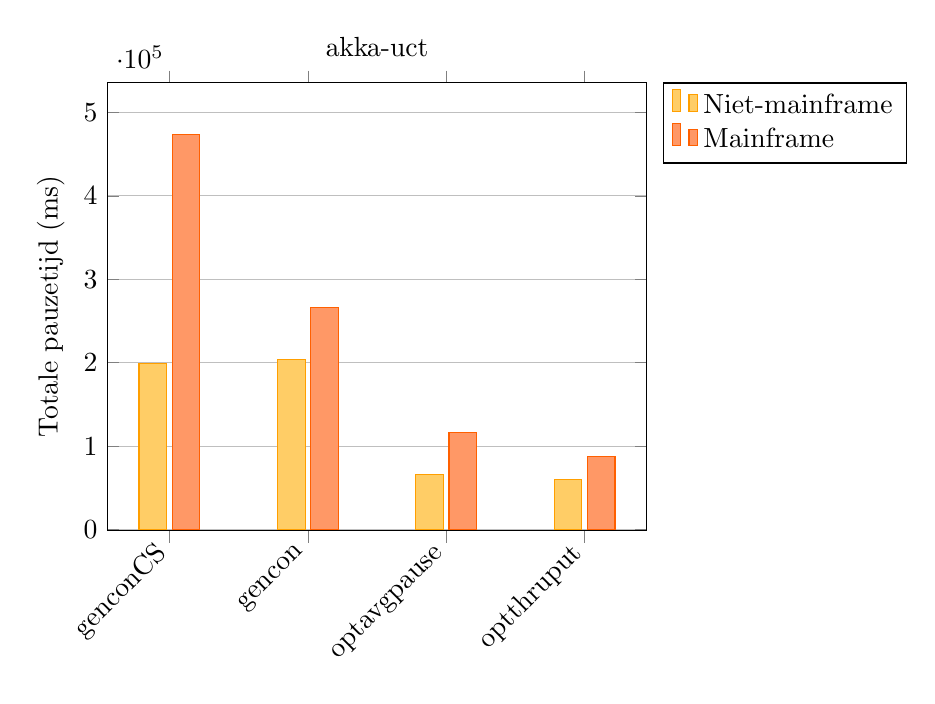
\begin{tikzpicture}
        \begin{axis}[
            title=akka-uct,
            ybar,
            enlargelimits=0.15,
            legend cell align=left,
            legend pos=outer north east,
            ylabel={Totale pauzetijd (ms)},
            ymajorgrids=true,
            symbolic x coords={genconCS,gencon,optavgpause,optthruput},
            x tick label style={rotate=45,anchor=east},
            ]
            \addplot[draw=orange!75!yellow,fill=orange!65!yellow!60!white] 
            coordinates {(genconCS,199200) (gencon,203429) (optavgpause,66527) (optthruput,60641)};
            \addplot [draw=orange!75!red,fill=orange!65!red!60!white] 
            coordinates {(genconCS,473857) (gencon,266216) (optavgpause,116630) (optthruput,87217)};
            \legend{Niet-mainframe,Mainframe}
        \end{axis}
    \end{tikzpicture}   
\end{figure}


%future-genetic pause-time
\begin{figure}[H]
    \caption[future-genetic totale pauzeertijd]{Vergelijkende tabel van de future-genetic programma, Garbage Collectors worden weergeven met hun totale pauzeertijd}  
    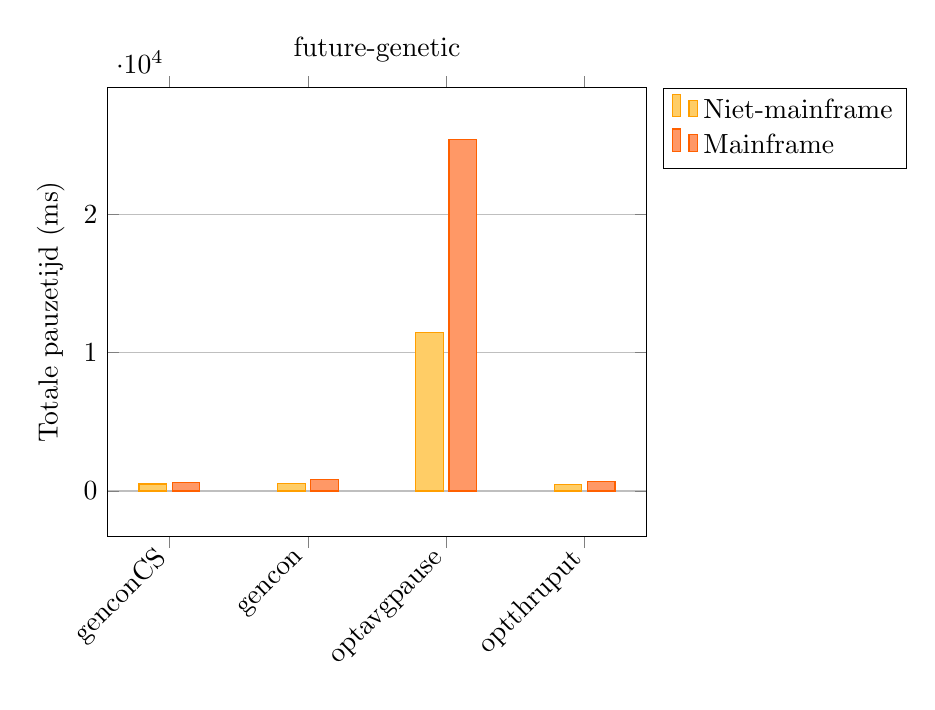
\begin{tikzpicture}
        \begin{axis}[
            title=future-genetic,
            ybar,
            enlargelimits=0.15,
            legend cell align=left,
            legend pos=outer north east,
            ylabel={Totale pauzetijd (ms)},
            ymajorgrids=true,
            symbolic x coords={genconCS,gencon,optavgpause,optthruput},
            x tick label style={rotate=45,anchor=east},
            ]
            \addplot[draw=orange!75!yellow,fill=orange!65!yellow!60!white] 
            coordinates {(genconCS,511) (gencon,561) (optavgpause,11463) (optthruput,473)};
            \addplot [draw=orange!75!red,fill=orange!65!red!60!white] 
            coordinates {(genconCS,596) (gencon,834) (optavgpause,25405) (optthruput,699)};
            \legend{Niet-mainframe,Mainframe}
        \end{axis}
    \end{tikzpicture}
\end{figure}
%dotty pause-time
\begin{figure}[H]
    \caption[dotty totale pauzeertijd]{Vergelijkende tabel van de dotty programma, Garbage Collectors worden weergeven met hun totale pauzeertijd} 
    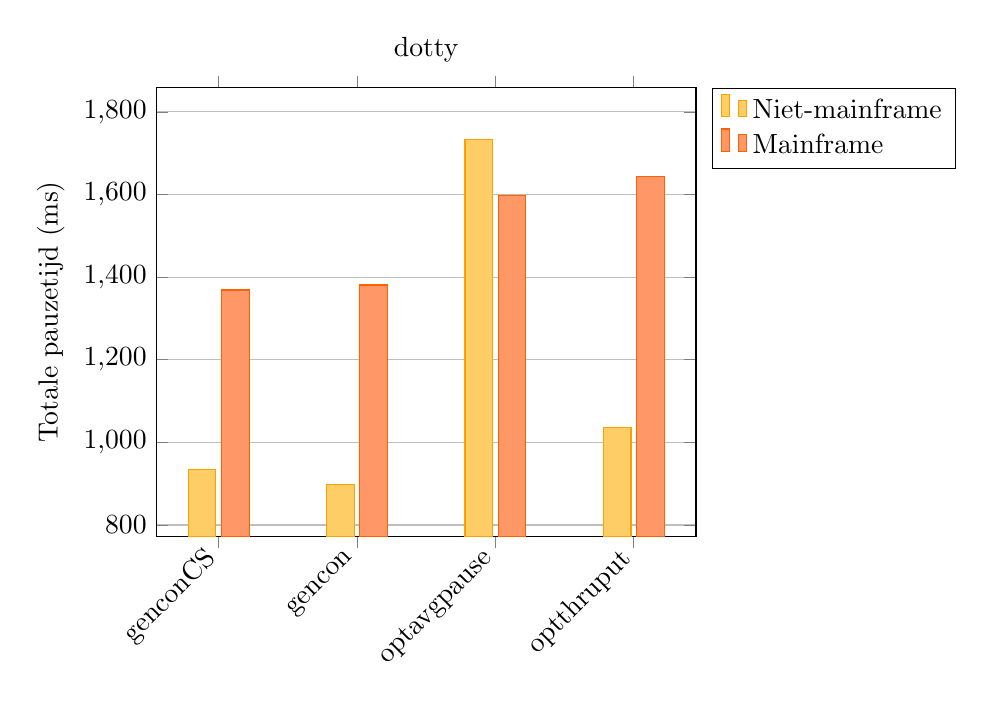
\begin{tikzpicture}
        \begin{axis}[
            title=dotty,
            ybar,
            enlargelimits=0.15,
            legend cell align=left,
            legend pos=outer north east,
            ylabel={Totale pauzetijd (ms)},
            ymajorgrids=true,
            symbolic x coords={genconCS,gencon,optavgpause,optthruput},
            x tick label style={rotate=45,anchor=east},
            ]
            \addplot[draw=orange!75!yellow,fill=orange!65!yellow!60!white] 
            coordinates {(genconCS,934) (gencon,898) (optavgpause,1733) (optthruput,1037)};
            \addplot [draw=orange!75!red,fill=orange!65!red!60!white] 
            coordinates {(genconCS,1369) (gencon,1381) (optavgpause,1598) (optthruput,1643)};
            \legend{Niet-mainframe,Mainframe}
        \end{axis}
    \end{tikzpicture}
\end{figure}

%finagle-chirper pause-time
\begin{figure}[H]
    \caption[finagle-chirper totale pauzeertijd]{Vergelijkende tabel van de finagle-chirper programma, Garbage Collectors worden weergeven met hun totale pauzeertijd} 
    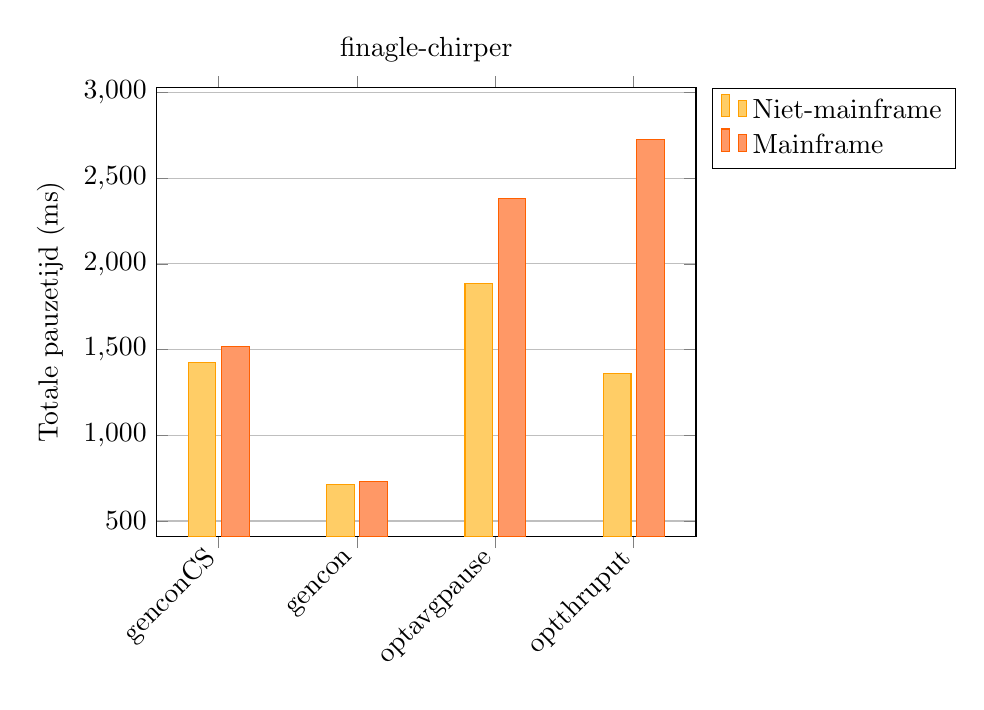
\begin{tikzpicture}
        \begin{axis}[
            title=finagle-chirper,
            ybar,
            enlargelimits=0.15,
            legend cell align=left,
            legend pos=outer north east,
            ylabel={Totale pauzetijd (ms)},
            ymajorgrids=true,
            symbolic x coords={genconCS,gencon,optavgpause,optthruput},
            x tick label style={rotate=45,anchor=east},
            ]
            \addplot[draw=orange!75!yellow,fill=orange!65!yellow!60!white] 
            coordinates {(genconCS,1426) (gencon,713) (optavgpause,1884) (optthruput,1360)};
            \addplot [draw=orange!75!red,fill=orange!65!red!60!white] 
            coordinates {(genconCS,1517) (gencon,728) (optavgpause,2379) (optthruput,2725)};
            \legend{Niet-mainframe,Mainframe}
        \end{axis}
    \end{tikzpicture}
\end{figure}

\section{Proportie ongepauzeerd}
De volgende grafieken geven de proportie dat een applicatie niet gepauzeerd werd door de GC weer van de mainframe en niet-mainframe Garbage Collection.
Dit in functie van de gekozen garbage collector policy, uitgedrukt in procent.

%akka-uct proportie ongepauseerd
\begin{figure}[H]
    
    \caption[akka-uct proportie ongepauseerd]{Vergelijkende tabel van de akka-uct programma, Garbage Collectors worden weergeven met de proportie van de applicatie tijd dat niet gepauzeerd werd door de Garbage Collection}
    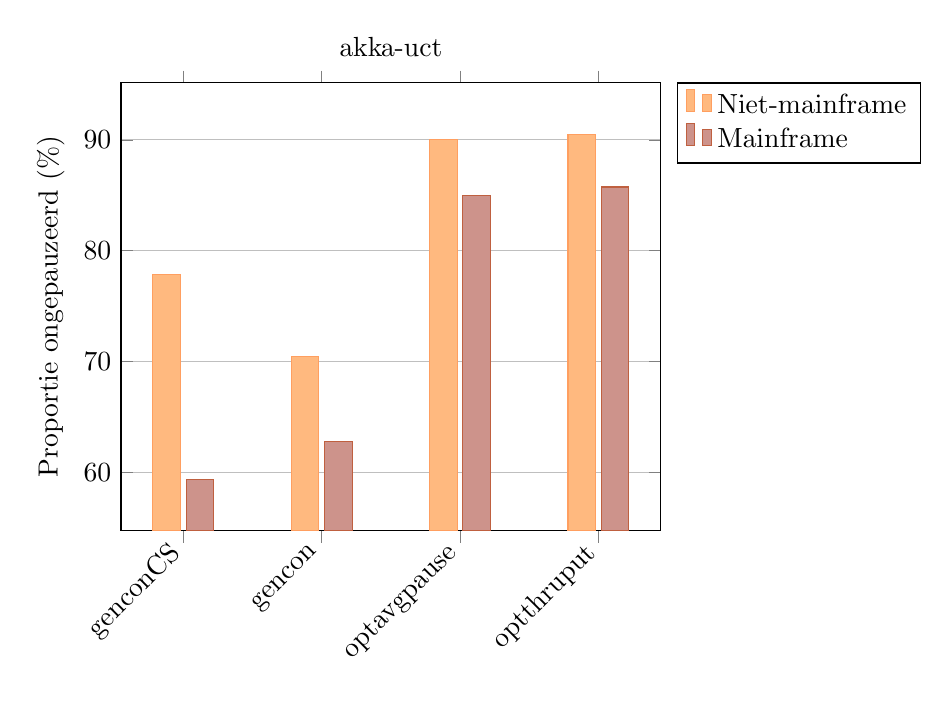
\begin{tikzpicture}
        \begin{axis}[
            title=akka-uct,
            ybar,
            enlargelimits=0.15,
            legend cell align=left,
            legend pos=outer north east,
            ylabel={Proportie ongepauzeerd (\%)},
            ymajorgrids=true,
            symbolic x coords={genconCS,gencon,optavgpause,optthruput},
            x tick label style={rotate=45,anchor=east},
            ]
            \
            \addplot[draw=orange!50!pink,fill=orange!70!pink!65!white] 
            coordinates {(genconCS,77.84) (gencon,70.47) (optavgpause,90.02) (optthruput,90.51)};
            \addplot[draw=orange!75!blue,fill=orange!70!blue!65!white] 
            coordinates {(genconCS,59.38) (gencon,62.81) (optavgpause,85.01) (optthruput,85.75)};
            \legend{Niet-mainframe,Mainframe}
        \end{axis}
    \end{tikzpicture}   
\end{figure}


%future-genetic proportie ongepauseerd
\begin{figure}[H]
    \caption[future-genetic proportie ongepauseerd]{Vergelijkende tabel van de future-genetic programma, Garbage Collectors worden weergeven met de proportie van de applicatie tijd dat niet gepauzeerd werd door de Garbage Collection}
    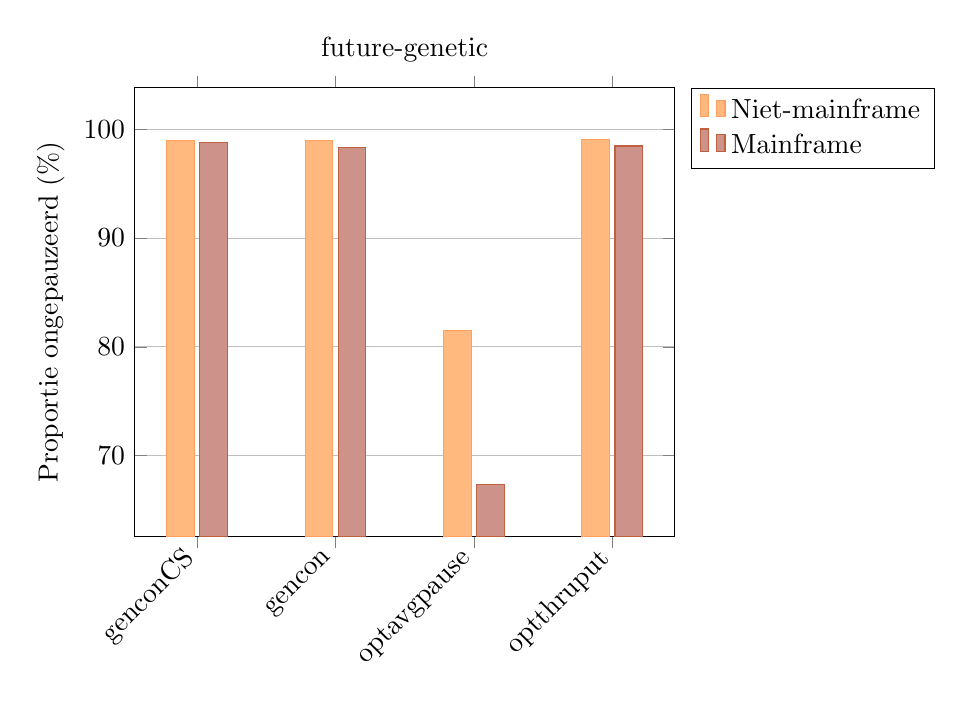
\begin{tikzpicture}
        \begin{axis}[
            title=future-genetic,
            ybar,
            enlargelimits=0.15,
            legend cell align=left,
            legend pos=outer north east,
            ylabel={Proportie ongepauzeerd (\%)},
            ymajorgrids=true,
            symbolic x coords={genconCS,gencon,optavgpause,optthruput},
            x tick label style={rotate=45,anchor=east},
            ]
            \
            \addplot[draw=orange!50!pink,fill=orange!70!pink!65!white] 
            coordinates {(genconCS,98.99) (gencon,98.94) (optavgpause,81.51) (optthruput,99.05)};
            \addplot[draw=orange!75!blue,fill=orange!70!blue!65!white] 
            coordinates {(genconCS,98.77) (gencon,98.33) (optavgpause,67.35) (optthruput,98.46)};
            \legend{Niet-mainframe,Mainframe}
        \end{axis}
    \end{tikzpicture}   
\end{figure}


%dotty proportie ongepauseerd
\begin{figure}[H]
    \caption[dotty proportie ongepauseerd]{Vergelijkende tabel van de dotty programma, Garbage Collectors worden weergeven met de proportie van de applicatie tijd dat niet gepauzeerd werd door de Garbage Collection}
    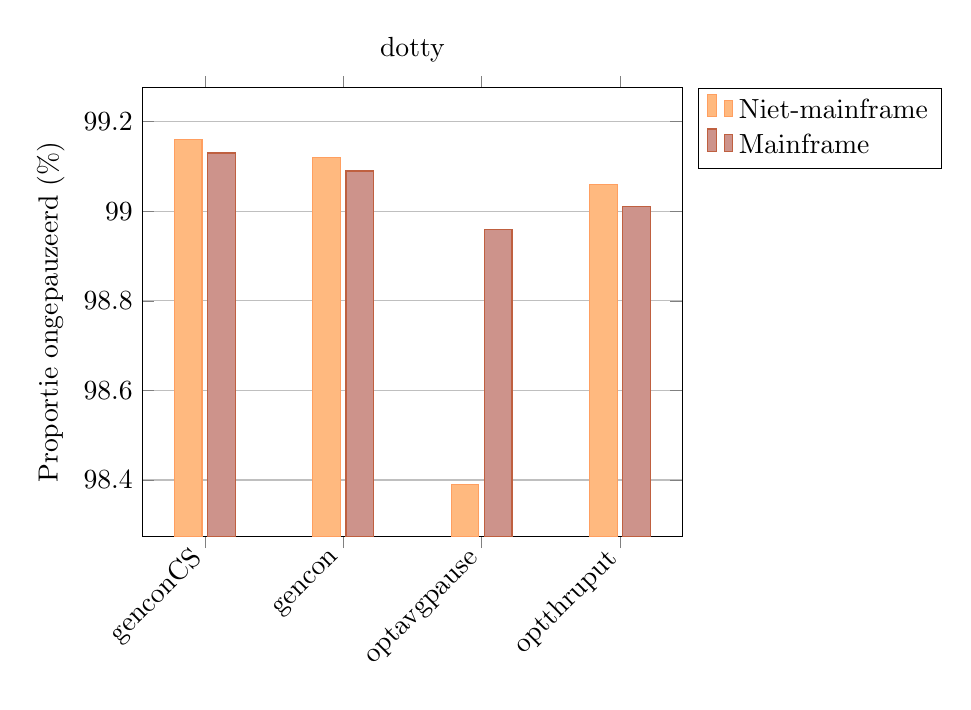
\begin{tikzpicture}
        \begin{axis}[
            title=dotty,
            ybar,
            enlargelimits=0.15,
            legend cell align=left,
            legend pos=outer north east,
            ylabel={Proportie ongepauzeerd (\%)},
            ymajorgrids=true,
            symbolic x coords={genconCS,gencon,optavgpause,optthruput},
            x tick label style={rotate=45,anchor=east},
            ]
            \
            \addplot[draw=orange!50!pink,fill=orange!70!pink!65!white] 
            coordinates {(genconCS,99.16) (gencon,99.12) (optavgpause,98.39) (optthruput,99.06)};
            \addplot[draw=orange!75!blue,fill=orange!70!blue!65!white] 
            coordinates {(genconCS,99.13) (gencon,99.09) (optavgpause,98.96) (optthruput,99.01)};
            \legend{Niet-mainframe,Mainframe}
        \end{axis}
    \end{tikzpicture}   
\end{figure}


%finagle-chirper proportie ongepauseerd
\begin{figure}[H]
    \caption[finagle-chirper proportie ongepauseerd]{Vergelijkende tabel van de finagle-chirper programma, Garbage Collectors worden weergeven met de proportie van de applicatie tijd dat niet gepauzeerd werd door de Garbage Collection}
    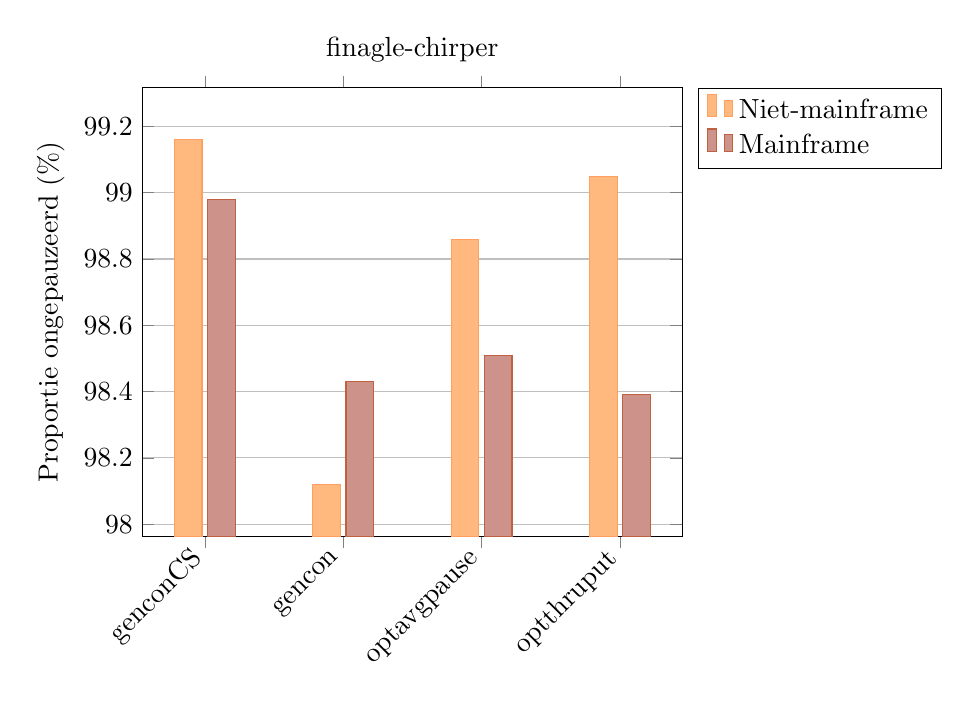
\begin{tikzpicture}
        \begin{axis}[
            title=finagle-chirper,
            ybar,
            enlargelimits=0.15,
            legend cell align=left,
            legend pos=outer north east,
            ylabel={Proportie ongepauzeerd (\%)},
            ymajorgrids=true,
            symbolic x coords={genconCS,gencon,optavgpause,optthruput},
            x tick label style={rotate=45,anchor=east},
            ]
            \
            \addplot[draw=orange!50!pink,fill=orange!70!pink!65!white] 
            coordinates {(genconCS,99.16) (gencon,98.12) (optavgpause,98.86) (optthruput,99.05)};
            \addplot[draw=orange!75!blue,fill=orange!70!blue!65!white] 
            coordinates {(genconCS,98.98) (gencon,98.43) (optavgpause,98.51) (optthruput,98.39)};
            \legend{Niet-mainframe,Mainframe}
        \end{axis}
    \end{tikzpicture}   
\end{figure}